\section{Smoothening of curves using the Box Kernel}

When smoothing a signal $f(t)$ using the box kernel $h(t)$, we compute the convolution:

$$
y(t) = (f * h)(t) = \int_{-\infty}^{\infty} f(\tau) h(t - \tau) d\tau
$$

For the rectangular kernel, this simplifies to:

$$
y(t) = \int_{t-T}^{t+T} f(\tau) d\tau
$$

This operation calculates the average value of $f(t)$ over a window of width $2T$ centered at point $t$. 
\newline\newline

This notion of "taking average" effectively "smoothens" or removes the noise of the curve it is convolved with. The box kernel acts as a low-pass filter, averaging out high-frequency noise while preserving the general shape of the signal. The choice of the kernel width $T$ is crucial; a larger $T$ results in greater smoothing but can distort finer features of the signal.

\subsection{Properties of Box Kernel Smoothing}

\subsubsection{Effect of Kernel Width}

The parameter $T$ controls the degree of smoothing:
\begin{itemize}
    \item Small $T$: Preserves more details but retains more noise
    \item Large $T$: Creates smoother curves but may obscure important features
\end{itemize}

\subsubsection{Limitations}

The box kernel produces a less smooth result compared to other kernels like Gaussian because of its abrupt cutoff at the boundaries. This creates a "choppy" appearance, especially in areas with sparse data.

\subsection{Some noisy curves and their convolved output}

Gaussian noise with mean $0$ and standard deviation $0.02$ is added to the original curve and then it is convolved with the box kernel.

\subsubsection{Noisy and Smoothed Sinusoid}
\begin{figure}[!ht]
\centering
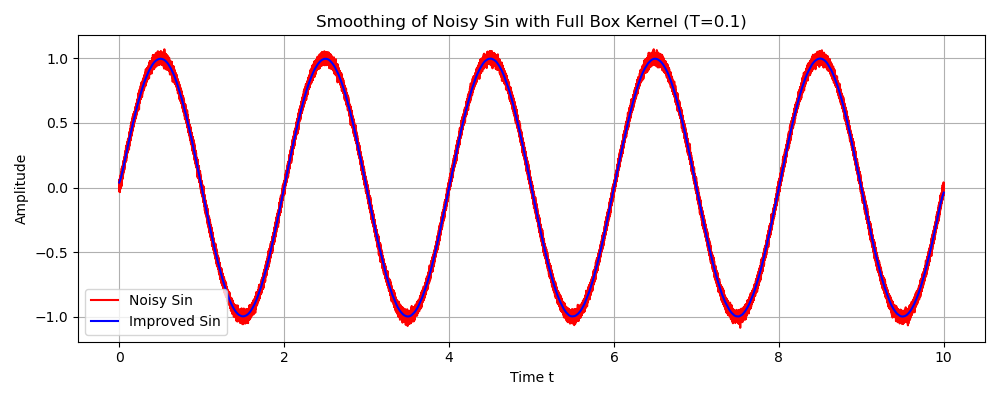
\includegraphics[width=0.8\textwidth]{codes/codes_sin_3_and_smoothening/figs/noisy_sin_plot.png}
\caption{Noisy Sinusoid and Smoothed Sinusoid}
\end{figure}
\FloatBarrier

\subsubsection{Noisy and Smoothed Step Function}
\begin{figure}[!ht]
\centering
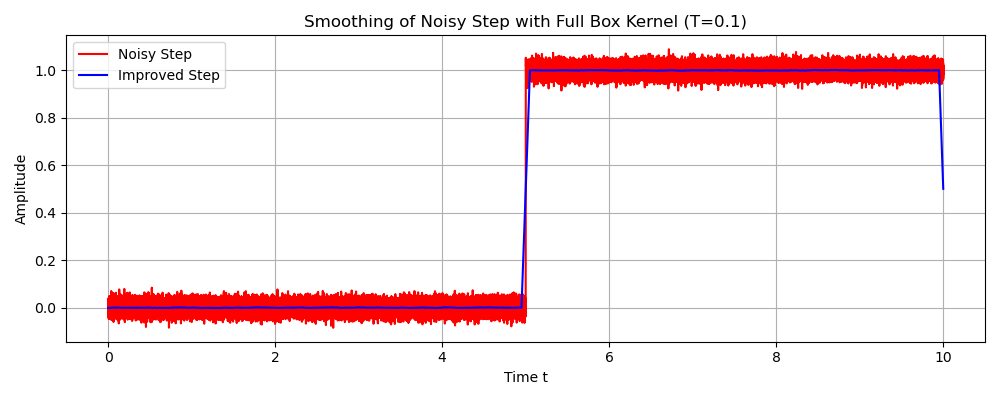
\includegraphics[width=0.8\textwidth]{codes/codes_sin_3_and_smoothening/figs/noisy_step_plot.png}
\caption{Noisy Step and Smoothed Step}
\end{figure}
\FloatBarrier

\subsubsection{Noisy and Smoothed Square Wave}
\begin{figure}[!ht]
\centering
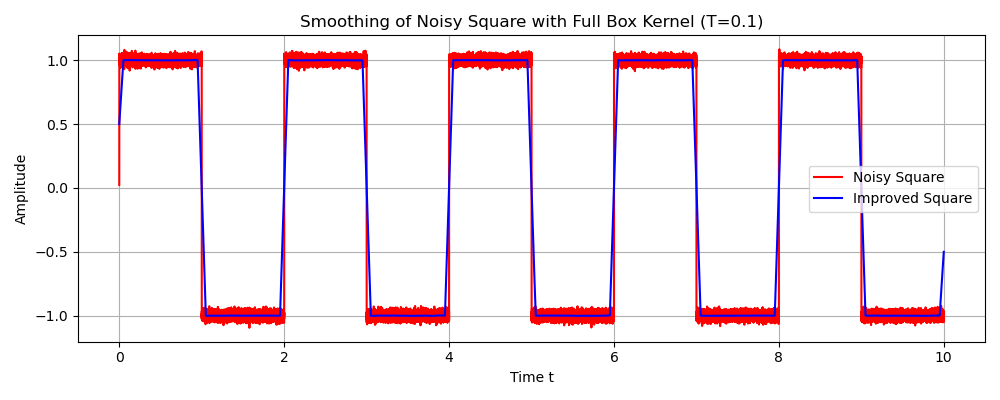
\includegraphics[width=0.8\textwidth]{codes/codes_sin_3_and_smoothening/figs/noisy_square_plot.png}
\caption{Noisy Square Wave and Smoothed Square Wave}
\end{figure}
\FloatBarrier

\subsubsection{Noisy and Smoothed Ramp}
\begin{figure}[!ht]
\centering
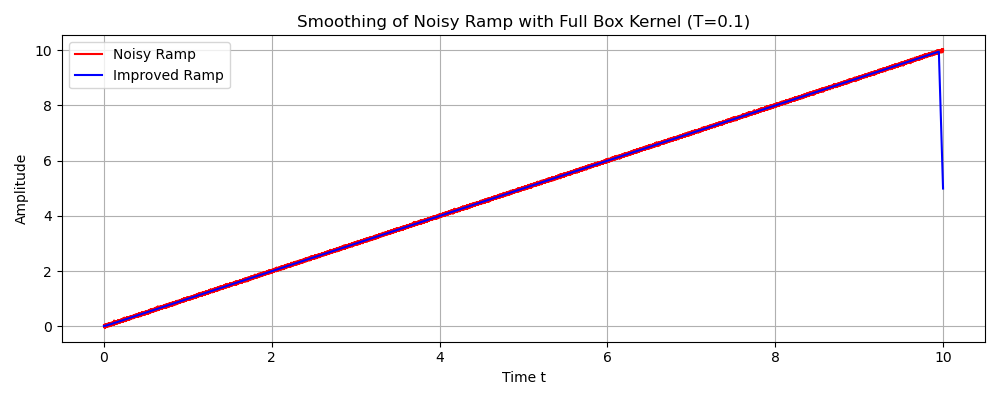
\includegraphics[width=0.8\textwidth]{codes/codes_sin_3_and_smoothening/figs/noisy_ramp_plot.png}
\caption{Noisy Ramp and Smoothed Ramp}
\end{figure}
\FloatBarrier

\subsubsection{Noisy and Smoothed Exponential Decay}
\begin{figure}[!ht]
\centering
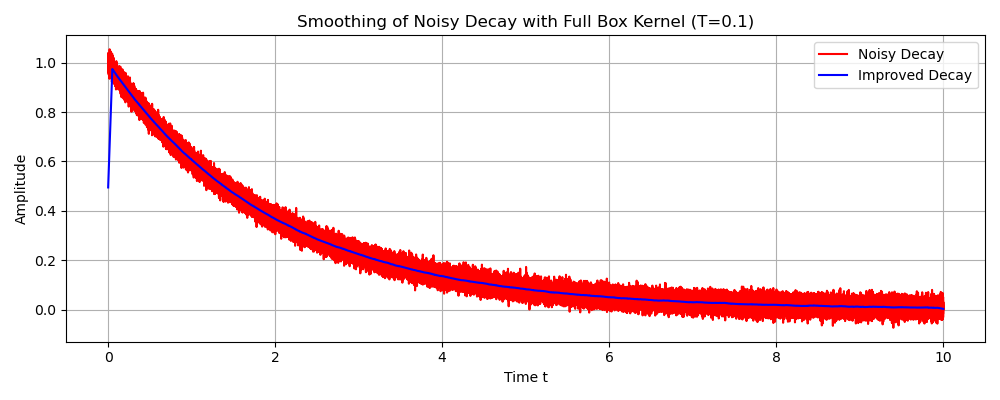
\includegraphics[width=0.8\textwidth]{codes/codes_sin_3_and_smoothening/figs/noisy_decay_plot.png}
\caption{Noisy Exponential Decay and Smoothed Exponential Decay}
\end{figure}
\FloatBarrier

\subsubsection{Noisy and Smoothed Gaussian Curve}
\begin{figure}[!ht]
\centering
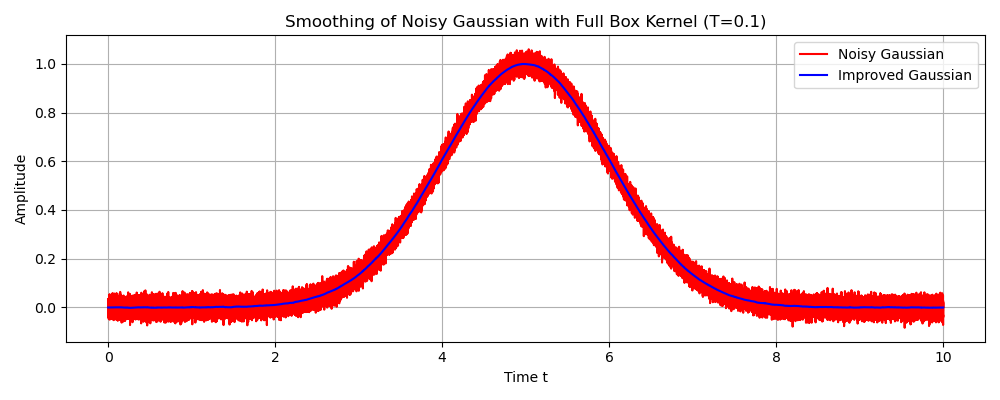
\includegraphics[width=0.8\textwidth]{codes/codes_sin_3_and_smoothening/figs/noisy_gaussian_plot.png}
\caption{Noisy Gaussian and Smoothed Gaussian}
\end{figure}
\FloatBarrier

\subsection{Smoothening out Gibbs phenomena in Fourier Reconstruction using Box Kernel}
Box kernel, in essence, smoothenes out noise. But an relatively interesting usecase would be to reduce the Gibbs Phenomena in the case of Fourier series.
\subsection{Square Wave Fourier Coefficients}
The square wave serves as an excellent example for demonstrating the Gibbs phenomenon. For a square wave alternating between $+1$ and $-1$ with period $2\pi$, the Fourier series is:

\begin{equation}
f(t) = \frac{4}{\pi} \sum_{n=1,3,5,...}^{\infty} \frac{1}{n} \sin(nt)
\end{equation}

\subsection{Convolving the square wave}

By linearity of the convolution operator,
\begin{align}
    (f * h)(t) = \frac{4}{\pi} \sum_{n=1,3,5,...}^{\infty} \left(\frac{2\sin{nT}}{n}\right) \frac{1}{n} \sin(nt) 
\end{align}
This alters the amplitude of the coefficients, which is obviously underisable. If we normalize this convolution amplitude factor, we get:
\begin{align}
    (f * h)(t) = \frac{4}{\pi} \sum_{n=1,3,5,...}^{\infty} \left(\frac{\sin{nT}}{nT}\right) \frac{1}{n} \sin(nt) 
\end{align}


\begin{figure}[!ht]
\centering
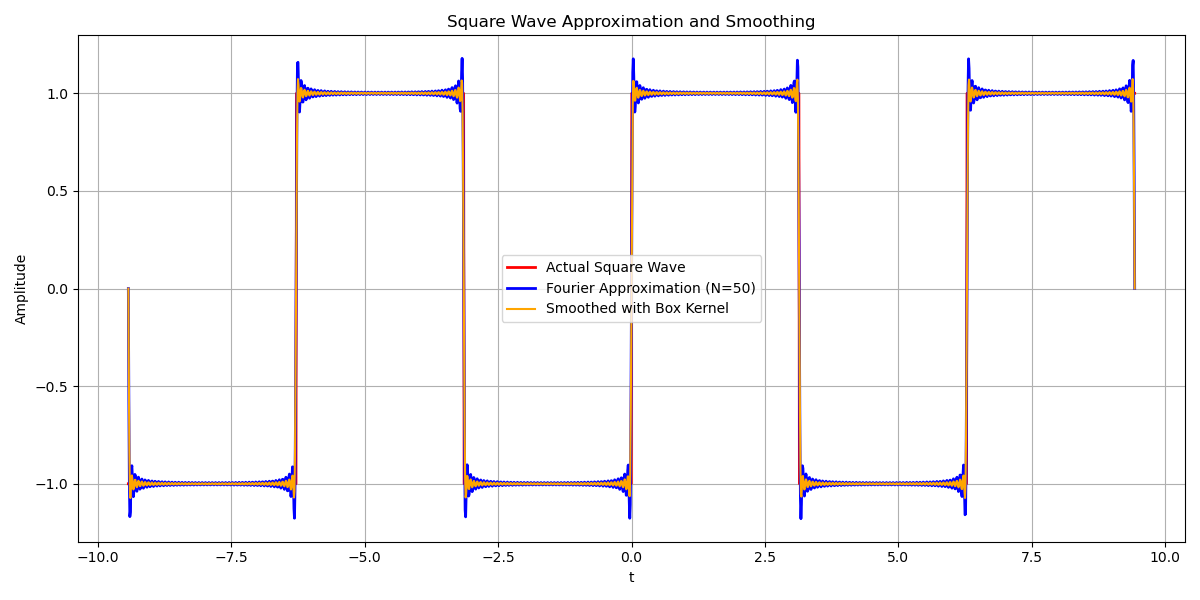
\includegraphics[width=0.8\textwidth]{codes/codes_sin_3_and_smoothening/figs/fourier_box_N50.png}
\caption{Slightly less Gibbs Phenomena in the Fourier Reconstruction at N = 50}
\end{figure}
\FloatBarrier

\begin{figure}[!ht]
\centering
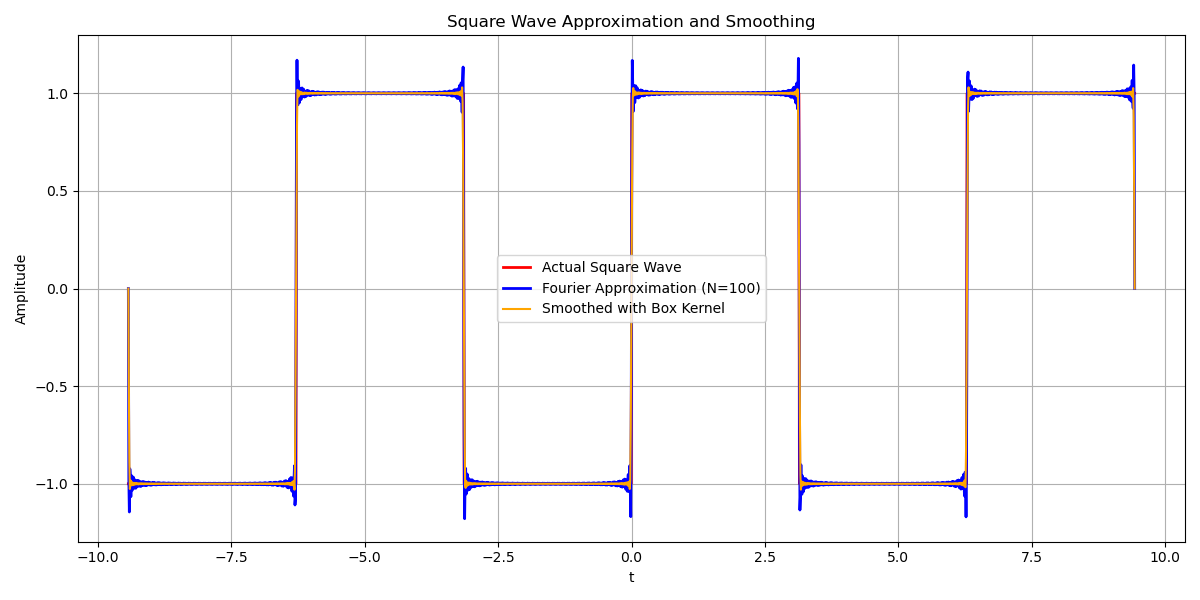
\includegraphics[width=0.8\textwidth]{codes/codes_sin_3_and_smoothening/figs/fourier_box_N100.png}
\caption{Slightly less Gibbs Phenomena in the Fourier Reconstruction at N = 100}
\end{figure}
\FloatBarrier
